\section{Dokumentformen}
		\begin{frame}
			\frametitle{Dokumentformen}
			\begin{itemize}
				\item Warum nicht Word?
				\item html
				\item pdf
			\end{itemize}
		\end{frame}

  \subsection{Warum nicht Word?}
  \only<article>{
    Das Web ist eine unvorstellbar große Sammlung von Dokumenten. Wenn man also im Internet surft, guckt man sich Dokumente an, die auf anderen Rechnern liegen. Nun haben doch alle Word \textendash{} warum also ein weiteres Format (html)? Es gibt dazu viele Argumente:
  } 

  \begin{frame}
    \frametitle{1. Dokumentgrößen}
    \begin{center}
      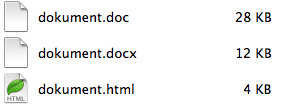
\includegraphics[width=6cm]{pics/Finder.png}
    \end{center}
  \end{frame}

  \begin{frame}
    \frametitle{die Dokumentauszeichnung am Beispiel ``Pages''}
      \begin{center}
        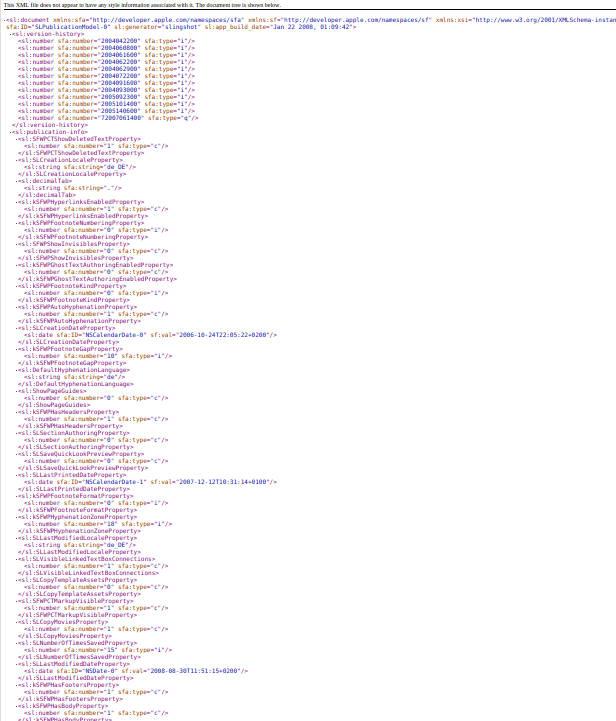
\includegraphics[height=6cm]{pics/auszeichnung.png}
        (noch 12 mal soviel\ldots)
      \end{center}
  \end{frame}

  \begin{frame}
    \frametitle{der Dokumentinhalt am Beispiel ``Pages''}
      \begin{center}
        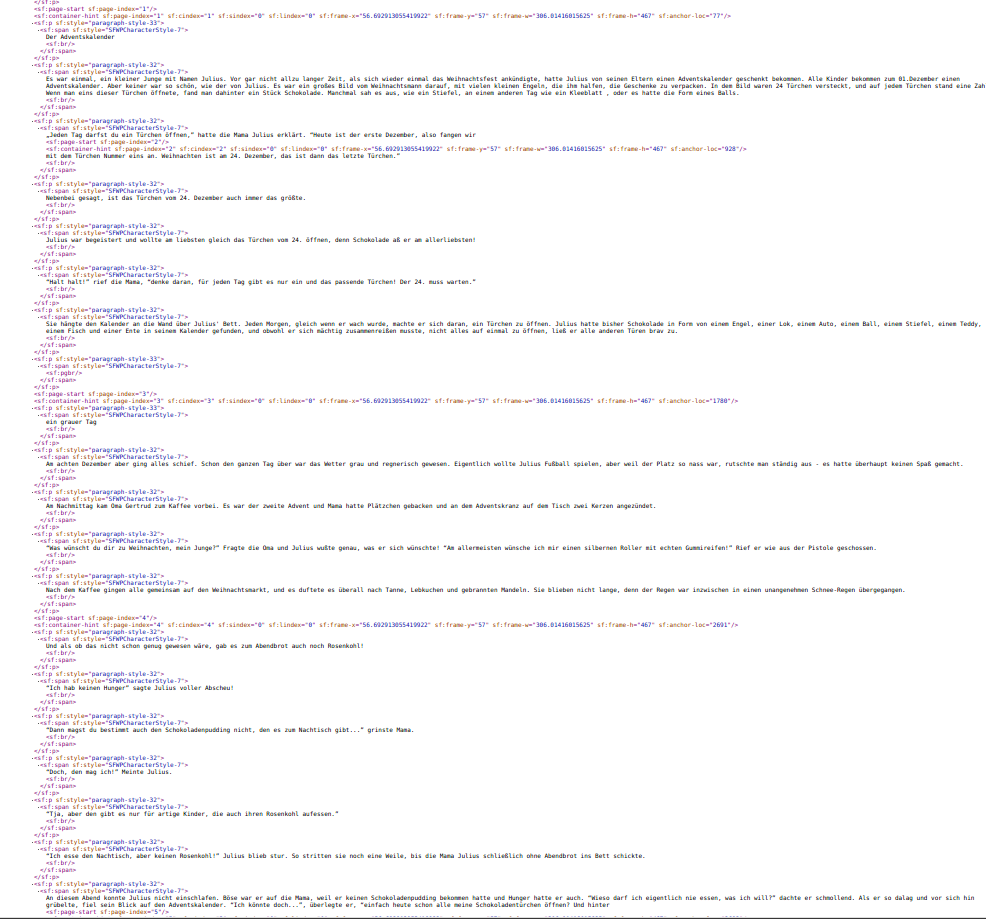
\includegraphics[height=6cm]{pics/der_eigentliche_text.png}
      \end{center}
  \end{frame}

  \only<article>{
    Bei der Übertragung über das Netz ist die Datei--Größe trotz ``dicker Leitungen'' nach wie vor entscheidend: Ein Word- Dokument mit dem gleichen Inhalt ist sieben mal (Word97-2003) bzw. dreimal (Word2007) grösser, als eine html-Datei gleichen Inhalts.  html ist ein Format, das sehr schlank ist und schnell übertragen werden kann. 
  }

  \begin{frame}
  \frametitle{2. frei verfügbares Format}
    Ein proprietäres Format wie .doc wird laufend verändert, wobei diese Veränderungen nicht dokumentiert werden. Wer das Dokument lesen will, muss die Software zum Lesen kaufen (können\ldots).

    
\includegraphics[height=3cm]{pics/pages-2011} \hfill 
\includegraphics[height=3cm]{pics/pages-2013}
  \end{frame}

  \only<article>{
    Webseiten sollten aber von jedem weltweit betrachtet werden können. 

    Ein weiterer Unterschied: Dokumente von Textverarbeitungen sind dafür gemacht, dass man sie leicht editieren kann. html- Dokumente dagegen sollen nach ihrer Erzeugung zunächst mal nur angezeigt, aber nicht bearbeitet werden. 

    Der Webbrowser schickt dazu eine Anfrage an den Server ``Reich mir mal die Seite /dokument.html rüber!''. Wenn die Seite vorhanden ist, gibt der Server sie heraus, sonst wird eine Fehlermeldung angezeigt. Der Webbrowserrückt die Seite raus, der Browser zeigt die Seite an - sobald man aber weiter surft, ist sie schon wieder vergessen (grundsätzlich\ldots{} Browser speichern heute Seiten in einem sogenannten Cache, damit sie beim nächsten Aufruf schneller kommen.). Bearbeiten kann man die Seite nicht. Mit speziellen Tools lässt sich der empfangene Code natürlich editieren, dann aber nur auf dem eigenen Rechner betrachten. Der Server wird es nicht erlauben, dass jeder einfach seine Änderungen auf ihm abspeichert.

    Und schliesslich gibt es für für Textverarbeitungen fest definierte Dokumentgrößen (A4 z.B.), Webseiten müssen aber auf den unterschiedlichsten Monitorgrößen angezeigt werden. Das bedeutet, dass z.B. Zeilenumbrüche flexibel sein müssen.
  }

  
  \subsection{html}
    \only<article>{
      html ist zunächst einmal keine Programmiersprache. Man kann keinen Rechner damit füttern und ihm das Ergebnis von $2 + 2$ entlocken. 

      html ist eine Auszeichnungssprache, die dazu dient, Inhalt zu formatieren. Dazu versieht der Programmierer den strukturierten Inhalt mit Tags --- eines zum Anfang und eines zum Ende des jeweiligen Bereichs. So kennzeichnen beispielsweise \lstinline{<p> </p>} einen Absatz. Zwischen den Tags steht dann der Inhalt.
    }
\begin{frame}[fragile]
\frametitle{eine einfache Seite}
  \begin{lstlisting}
    <html>
      <head>
        <title>Der Hase und der Baum</title>
      </head>
      <body>
        <h1>Der Hase und der Baum</h1>
        <h2>Kapitel 1: Der Hase</h2>
        <p>Meister Lampe hoppelt über ein Feld.</p>
        <h2>Kapitel2: In der Werkstatt</h2>
        <p>Herr K. bestellt eine Knautschzone.</p>
      </body>
    </html>
  \end{lstlisting}
\end{frame}

\begin{frame}
\frametitle{\ldots sieht so aus:}
  \begin{center}
    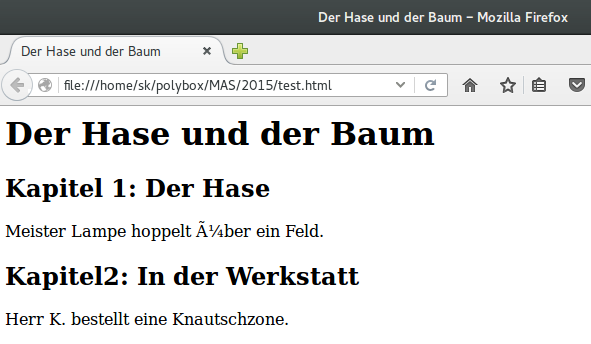
\includegraphics[width=0.8\textwidth]{pics/testseite.png}
  \end{center}
\end{frame}

\begin{frame}[fragile]
\frametitle{\ldots mit Umlauten:}
  \begin{lstlisting}
    <html>
      <head>
      <meta charset="utf-8" />
        <title>Der Hase und der Baum</title>
      </head>
      <body>
        <h1>Der Hase und der Baum</h1>
        <h2>Kapitel 1: Der Hase</h2>
        <p>Meister Lampe hoppelt über ein Feld.</p>
        <h2>Kapitel2: In der Werkstatt</h2>
        <p>Herr K. bestellt eine Knautschzone.</p>
      </body>
    </html>
  \end{lstlisting}
\end{frame}

\begin{frame}
\frametitle{\ldots sieht so aus:}
  \begin{center}
    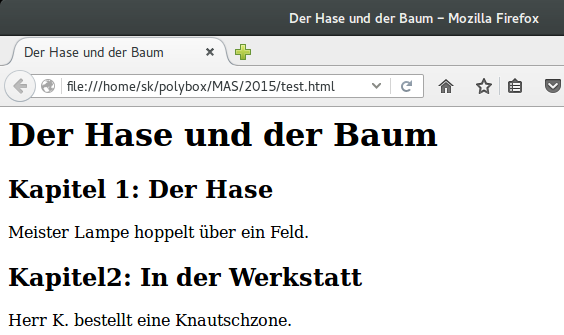
\includegraphics[width=0.8\textwidth]{pics/testseite-utf8.png}
  \end{center}
\end{frame}

\only<article>{
  \pagebreak
}

\begin{frame}
\frametitle{So soll es sein:}
  \begin{center}
    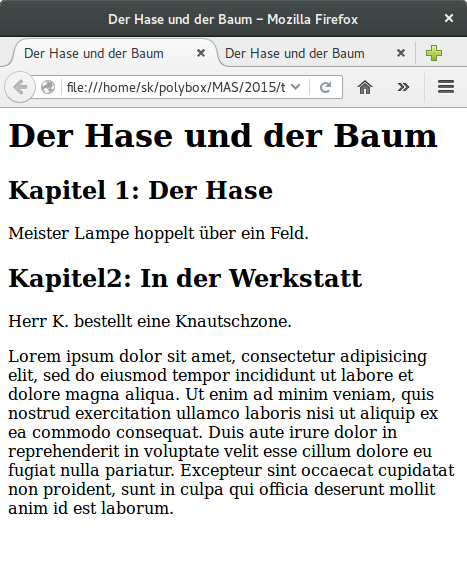
\includegraphics[width=0.4\textwidth]{pics/testseite-gut.png}
  \end{center}
\end{frame}

\begin{frame}
\frametitle{So soll es nicht sein!}
  \begin{center}
    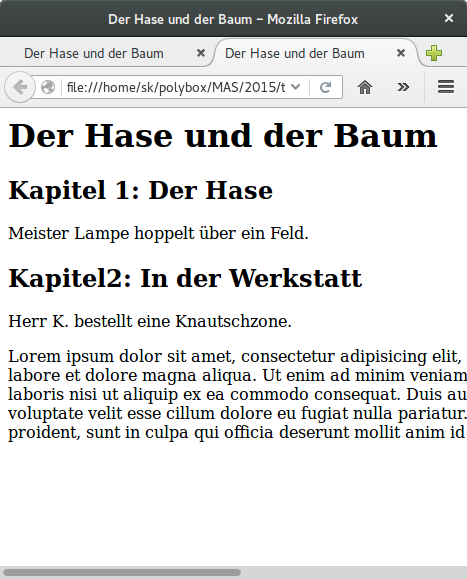
\includegraphics[width=0.4\textwidth]{pics/testseite-feste_breite.png}
  \end{center}
\end{frame}

  \subsection{pdf}
  \only<article>{
    Wenn man ein Dokument mit festem Layout veröffentlichen möchte, bietet sich PDF an. Es ist frei verfügbar, kann also von jedem gelesen werden, und sieht immer gleich aus. Wie auch Webseiten lässt es sich (eigentlich) nicht vom Empfänger verändern.
    }

\begin{frame}
\frametitle{Wieder die Dokumentgrösse:}
  \begin{center}
    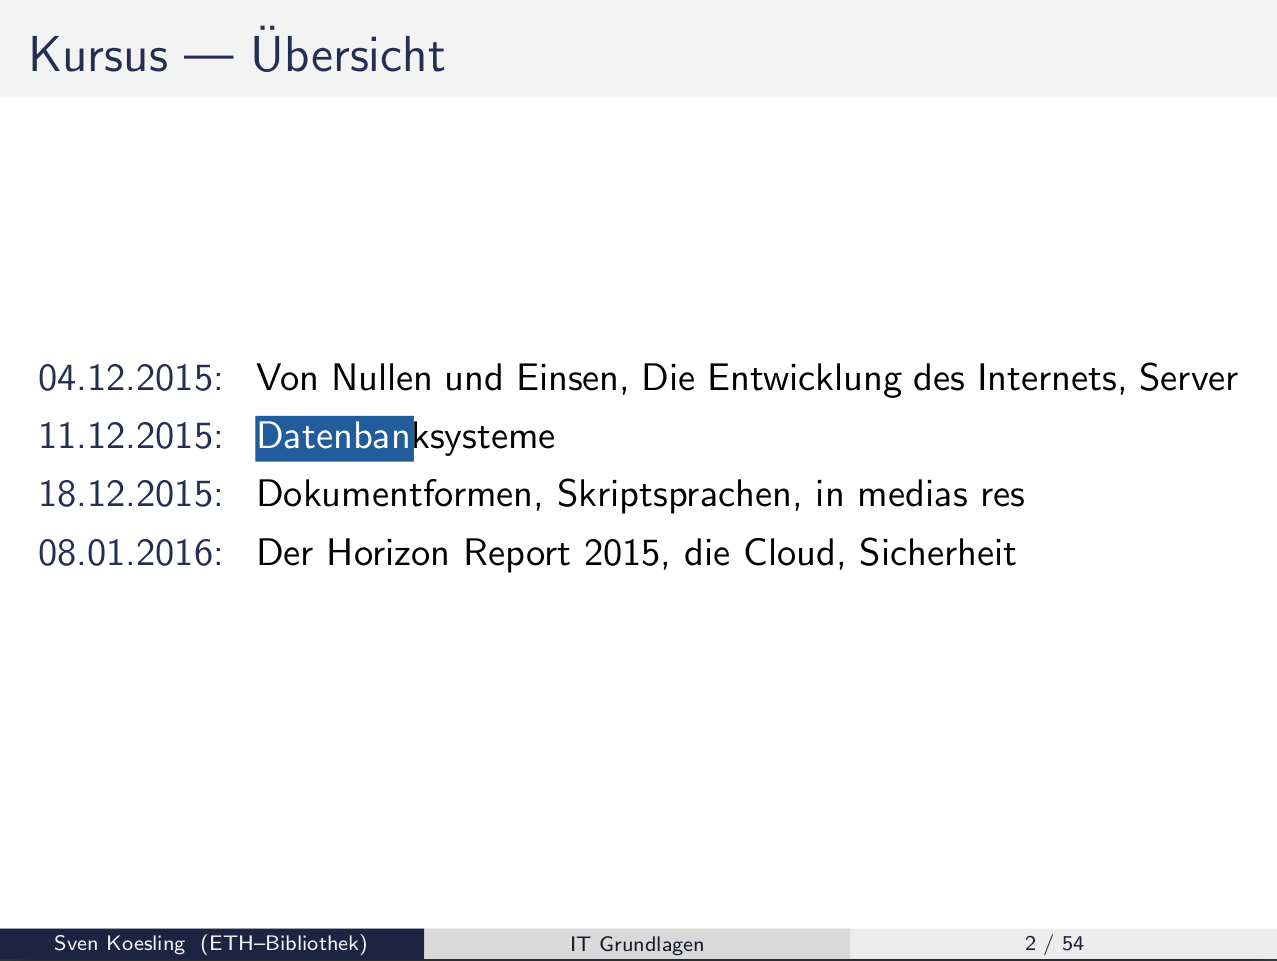
\includegraphics[width=0.6\textwidth]{pics/copy-paste.png}

    als Bild: 72.2 kB (72'224 Bytes)\\
    als PDF: 35.9 kB (35'880 Bytes)
  \end{center}
\end{frame}

\begin{frame}
\frametitle{Fazit: Welche Form wofür?}
    \textbf{Textverarbeitung:} Alles zum Weiterverarbeiten

    \textbf{html:} Inhalt geht über Form

    \textbf{PDF:} Form soll erhalten bleiben
\end{frame}

\begin{frame}
\frametitle{alles Quatsch?}
\begin{theorem}
  Im Web liest doch niemand mehr. Da sollte man nur knappe Infos unterbringen.
\end{theorem}
\end{frame}

\section{Exkurs: stateless}
  \only<article>{
    Ein Problem bei der Entwicklung von Web--Apps war, dass ein Webserver eigentlich nichts vom User weiss. Er liefert die geforderte Webseite aus und hat dann den User schon wieder ``vergessen''.
  }
\begin{frame}
\frametitle{http is stateless}
  
\includegraphics[width=0.8\textwidth]{pics/whatsyournameagain}
\end{frame}

\begin{frame}[fragile]
  \begin{quote}
    HTTP is a stateless protocol. A stateless protocol does not require the server to retain information or status about each user for the duration of multiple requests.

    But some web applications may have to track the user's progress from page to page, for example when a web server is required to customize the content of a web page for a user. Solutions for these cases include:
    \begin{itemize}
      \item the use of HTTP cookies.
      \item server side sessions,
      \item hidden variables (when the current page contains a form), and
      \item URL-rewriting using URI-encoded parameters, e.g., \lstinline{/index.php?session_id=some_unique_session_code}.
    \end{itemize}
    \hfill(wikipedia)
  \end{quote}
\end{frame}

  \only<article>{
    Um das zu ändern gibt es verschiedene Techniken wie z.B. Cookies und Sessions. Dabei handelt die Web--App einen eindeutigen Identifier aus und kann so wiederkehrende User identifizieren. ``Dank'' der Werbeindustrie wurden diese Techniken so weit optimiert, dass wir im Internet gläsern sind. Man kann feststellen, woher wir kommen, welche Seiten wir gesehen haben, welche wir wegklicken, wie lange wir wo verweilt haben und, und, und. 
  }

\begin{frame}
\frametitle{privacy?}
  \begin{quote}
    You have zero privacy anyway. Get over it. \hfill(Scott McNealy, Sun Microsystems, 1999)
  \end{quote}
\end{frame}

\section{Exkurs: Themen für die Postersession}
  
  \only<beamer>{
    \begin{frame}
      \frametitle{Exkurs: Themen für die Postersession}
      \begin{itemize}
        \item Google und Bibliotheken
        \item Die Zusammenarbeit von Fachabteilungen und IT
        \item Der Horizonreport 2015 Library Edition
      \end{itemize}
    \end{frame}
  }

  \begin{frame}
    \frametitle{Google und Bibliotheken}
      \begin{itemize}
        \item Welche Gemeinsamkeiten und welche Unterschiede bestehen in den Anforderungen an Google und an eine Bibliothek?
        \item Auf welche Datenbanktechnologien setzt Google?
        \item Welches Business wäre eventuell für den Wissenstransfer besser geeignet, als Google?
    \end{itemize}
  \end{frame}

  \begin{frame}
    \frametitle{Die Zusammenarbeit von Fachabteilungen und IT}
      \begin{itemize}
        \item Beschreiben Sie eine typische Situation mit Differenzen aus Sicht der Fachabteilung.
        \item Beschreiben Sie die gleiche Situation so, wie Sie sich die Sicht der IT vorstellen.
        \item Was wäre aus Ihrer Sicht der Idealzustand?
      \end{itemize}
  \end{frame}

  \begin{frame}
    \frametitle{Der Horizonreport 2015 Library Edition}
      \begin{itemize}
        \item Beschreiben sie die Auswirkungen einer möglichen zukünftigen technischen Entwicklung auf Bibliotheken.
        \item Welche Rolle spielt die Strategie in dieser Entwicklung?
        \item Was müsste man aus Ihrer Sicht für Bibliotheken erfinden?
      \end{itemize}
  \end{frame}

\section{Skriptsprachen}

\begin{frame}
  \begin{center}
    
\includegraphics[width=1\textwidth]{pics/scriptsprachen-logos}
  \end{center}
\end{frame}

\only<article>{
    Wärend man mit Auszeichnungssprachen wie z.B. html oder \LaTeX\ Dokumente formatiert, dienen Skriptsprachen wie Perl, Ruby oder Javascript dazu, einfache, wiederkehrende Aufgaben am Computer zu übernehmen.

    Beim Publishing von Aleph erhalten wir beispielsweise unzählige komprimierte Dateien, die ihrerseits unzählige XML-Dateien enthalten. Jede dieser XML-Dateien enthält einen Datensatz.
  }

\begin{frame}
  \frametitle{Das erste Programm}
    \begin{center}
    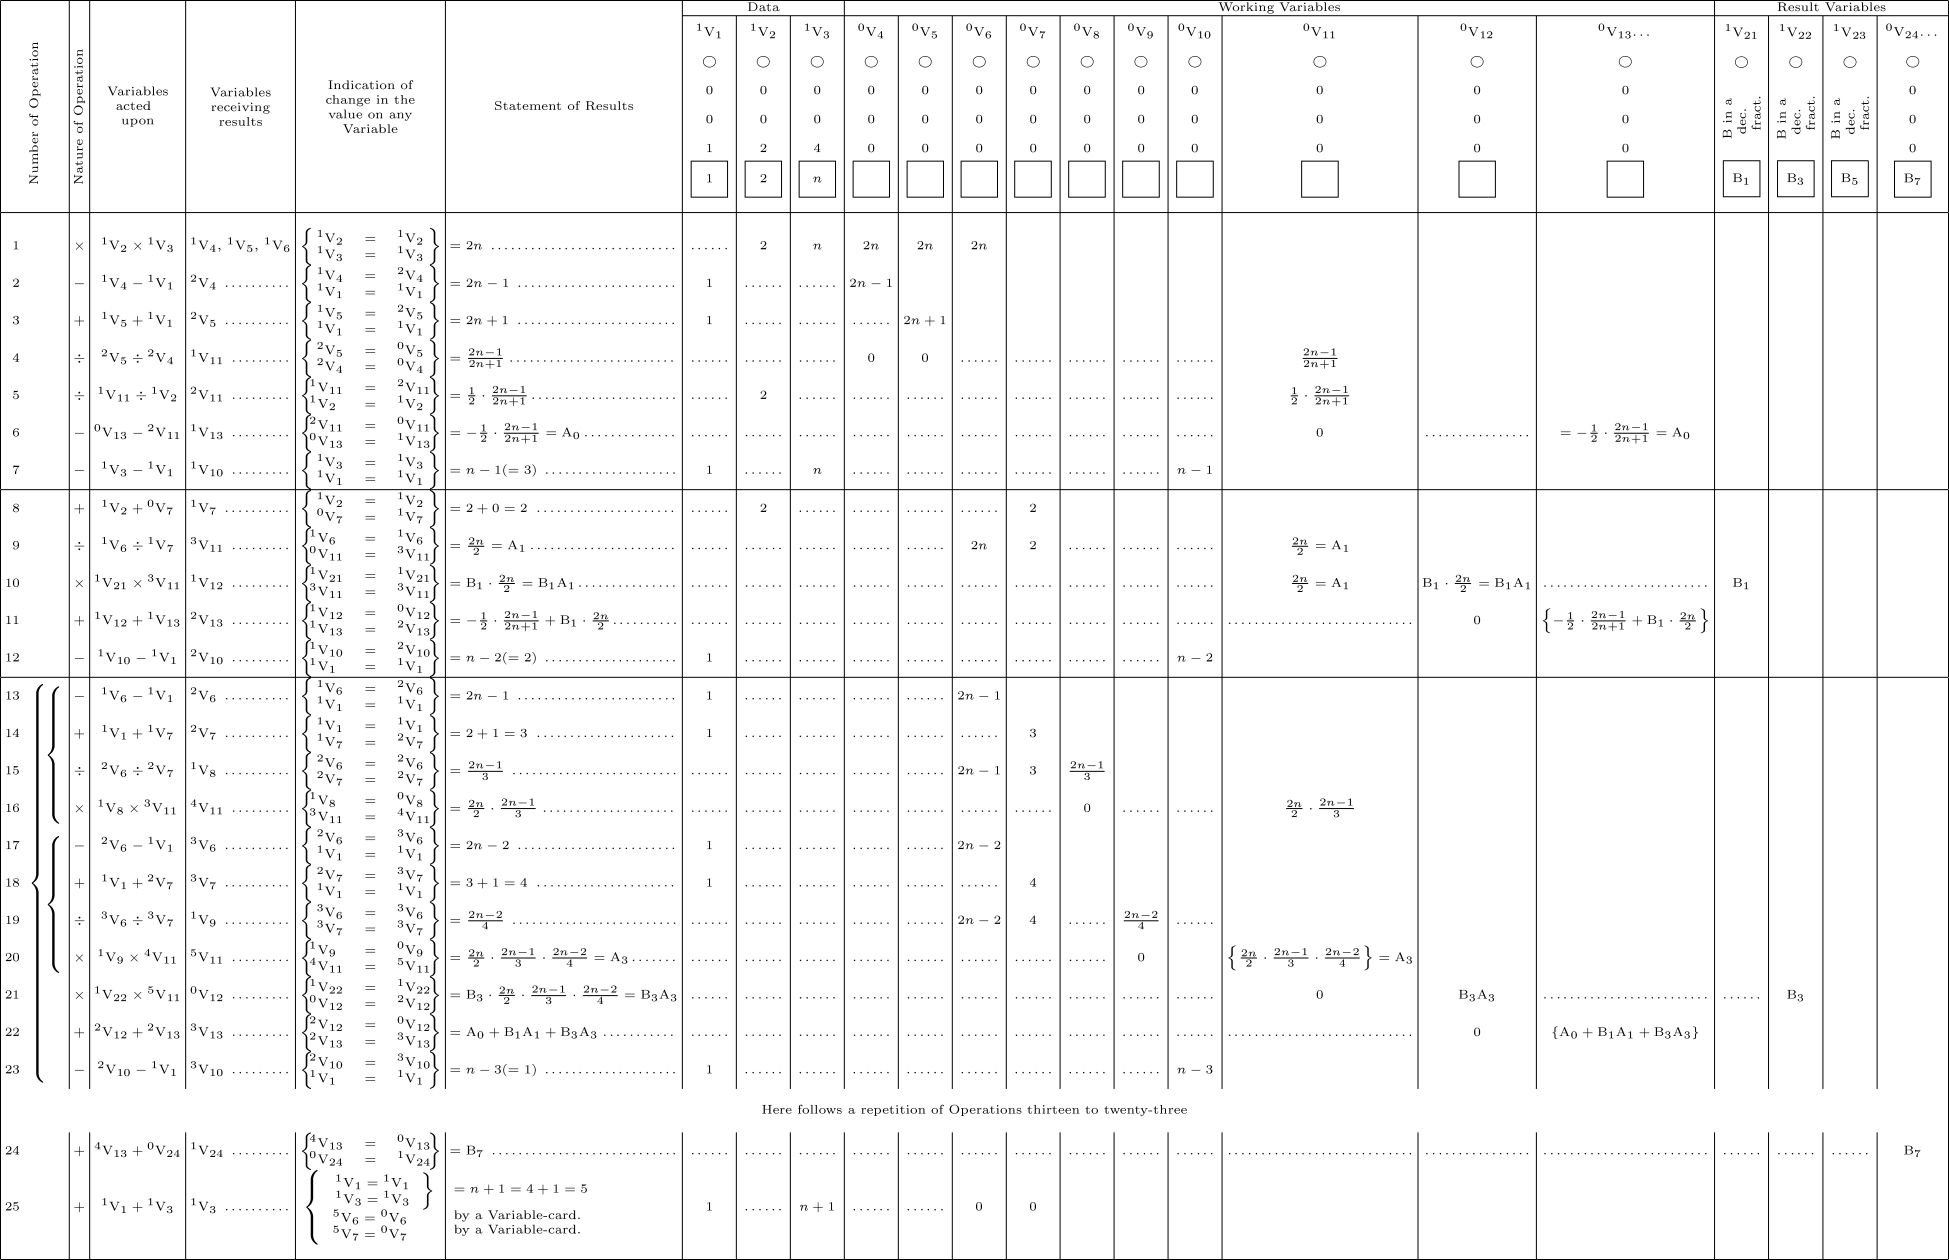
\includegraphics[width=0.8\textwidth]{pics/dasersteprogramm.png}
    \end{center}
\end{frame}

\begin{frame}[fragile]
  \frametitle{Ein Programm}
  Das folgende Skript (Auszug) dient zum Durchsuchen von tar-files:
  
  \begin{lstlisting}
  Dir.entries("./").each do |tarname|
  if tarname =~ /tar\.gz$/
    tarinhalt = %x(tar -tzf #{tarname}) 
    tarinhalt.each_line do |dateiname|
      dateiname.chomp!
     if dateiname =~ /#{suchstring}/
      puts "#{suchstring} kommt in #{dateiname} im Archiv #{tarname} vor"

      puts "Soll die Datei extrahiert werden: j/N"
      antwort = gets
  \end{lstlisting}

  \ldots
\end{frame}

  \subsection{serverseitige Skriptsprachen}
  \only<article>{
    Die Einteilung in server--- und clientseitige Skriptsprachen ist ein bisschen willkürlich, macht aber bestimmte Konzepte gut deutlich. Grundsätzlich könnten alle Skriptsprachen sowohl auf dem Client als auch auf dem Server vorhanden sein.

    Hier soll es aber darum gehen, dass --- je nachdem, auf welcher Seite das Skript läuft --- bestimmte Funktionen möglich sind, andere eben nicht.
  }
  \subsection{clientseitige Skriptsprachen}
  \only<article>{
    dienen dazu, mit dem Server zu kommunizieren, Funktionen auf dem Client auszuführen, die Webseite beim User zu manipulieren
  }
  \subsection{regular Expressions}



\section{in medias res}
\begin{frame}
\frametitle{Wir setzen das Gelernte zusammen}
  Wie entstehen dynamische Webseiten? 
\end{frame}
